% $Header: /Users/joseph/Documents/LaTeX/beamer/solutions/conference-talks/conference-ornate-20min.en.tex,v 90e850259b8b 2007/01/28 20:48:30 tantau $

\documentclass[utf8,t,compress,xcolor=svgnames,handout]{beamer}

%\usepackage{pgfpages}
%\pgfpagesuselayout{4 on 1}[a4paper,landscape,border shrink=5mm]

\usepackage{calc}
\usepackage{ifthen}
\usepackage[sfdefault]{cabin}
\usepackage[T1]{fontenc}
\usepackage[english]{babel}	   % English hyphenation
\usepackage{csquotes}		 % Multilingual quotes
\usepackage[babel]{microtype}    % Awesome microtyping

\usepackage{booktabs}    % Better tables
%\usepackage{tablefootnote}    % Allows footnotes in tables
\usepackage{commath}    % Differential operators
\usepackage{bm}
\usepackage{multirow}

% Extra symbols
\usepackage{wasysym}
\newcommand\pro{\item[\textbf{\CheckedBox}]}
\newcommand\con{\item[\textbf{\XBox}]}
\newcommand\neu{\item[\textbf{\Square}]}

% Graphics
\usepackage{graphicx}
\DeclareGraphicsExtensions{.pdf,.png,.jpg}
\graphicspath{{img/}}    % Central repository for images
\usepackage{emerald}
\usepackage{tikz}
\usepackage{pgf}
\usepackage{pgffor}
\usepackage{mathrsfs}
\usetikzlibrary{arrows,shapes.geometric,shapes.misc}

% Bibliography
\usepackage[backend=biber,style=alphabetic,sorting=ydnt]{biblatex}
\addbibresource{thesis.bib}

% Set fonts
\setbeamerfont{my frametitle}{size=\Large}
\setbeamerfont{framesubtitle}{size=\large}
\setbeamerfont{title}{size=\huge}
\setbeamerfont{subtitle}{size=\Large}
\setbeamerfont{author}{size=\large}
\setbeamerfont{date}{size=\large}
\setbeamerfont{institute}{size=\large}

%%% Frametitle
%\setbeamertemplate{frametitle}{
%	\begin{beamercolorbox}{frametitle}
%		\vskip0.75em
%		\usebeamerfont{frametitle}
%		\insertframetitle \\
%		\usebeamerfont{framesubtitle}\insertframesubtitle
%	\end{beamercolorbox}
%}
%
%%% remove navigation symbols
%\setbeamertemplate{navigation symbols}{}
%
%%% Date in the Corner
%\setbeamertemplate{headline}{
%	\rotatebox{30}{
%		\ifx\insertdate\empty\else        
%		\hspace*{0.25cm}\insertshortdate\hspace*{0.5cm}
%		\fi
%	}
%	\vspace*{-1cm}
%}


% Figure styles
\tikzset{
	header/.style={
		% The shape:
		rectangle,minimum size=6mm,
		% The rest
		draw=black!10,
	}}
	
	\tikzset{
		term/.style={
			% The shape:
			shape=rectangle,rounded corners=3mm,
			% The size:
			minimum size=6mm,
			% The border:
			very thick,
			draw=red!50!black!50, % 50% red and 50% black,
			% and that mixed with 50% white
			% The filling:
			%			top color=white, % a shading that is white at the top...
			%			bottom color=red!50!black!20 % and something else at the bottom
		}}
		
		\tikzset{
			nterm/.style={
				% The shape:
				rectangle,minimum size=6mm,rounded corners=3mm,
				% The rest
				very thick,draw=black!30,
				%			top color=black!05,bottom color=black!10,
			}}
			
			
			\title{Pricing exotic path-dependent options}
			\subtitle{The Singular Points method}
			\date[2015-10-23]{23\textsuperscript{rd} October, 2015}
			\institute[MathMods]{MathMods\\{Universita degli Studi dell'Aquila}}
			\author[Sudip Sinha]{Sudip Sinha}

% This file is a solution template for:

% - Talk at a conference/colloquium.
% - Talk length is about 20min.
% - Style is ornate.



% Copyright 2004 by Till Tantau <tantau@users.sourceforge.net>.
%
% In principle, this file can be redistributed and/or modified under
% the terms of the GNU Public License, version 2.
%
% However, this file is supposed to be a template to be modified
% for your own needs. For this reason, if you use this file as a
% template and not specifically distribute it as part of a another
% package/program, I grant the extra permission to freely copy and
% modify this file as you see fit and even to delete this copyright
% notice. 


\mode<presentation>
{
  \usetheme{Warsaw}
  % or ...

  \setbeamercovered{transparent}
  % or whatever (possibly just delete it)
}



\title{Pricing exotic path-dependent options}
\subtitle{The Singular Points method \cite{Gaudenzi2010,Gaudenzi2011}}
\date[2015-10-23]{23\textsuperscript{rd} October, 2015}
\institute[MathMods]{MathMods\\{Università degli Studi dell'Aquila}}
\author[Sudip Sinha]{Sudip Sinha\\{Supervisor: Prof. Fabio Antonelli}}
\subject{Mathematical Finance}


\begin{document}
	
	\begin{frame}[plain]
		\maketitle
	\end{frame}
	
	
	\section{Motivation}
	
	\begin{frame}{(Financial) Market models: introduction}
		\begin{itemize}
			
			\item Financial assets
			\begin{itemize}
				\item basic assets
				\begin{description}
					\item[riskless (deterministic)] treasury bonds: $ S_t^0 = e^{rt} $
					\item[risky (stochastic)] stocks: $ (S_t)_t $, parameter $ \sigma $ characterises risk
				\end{description}
				\item derivatives -- contracts on other assets (\emph{underlying}), till \emph{maturity} $ T $
				\begin{description}
					\item[futures] symmetric risk
					\item[options] asymmetric risk -- historically used for insurance
				\end{description}
			\end{itemize}
			
			\item Problem: pricing derivatives
			
			\item Assumptions
			\begin{itemize}
				\item viable / no arbitrage / no free lunch
				\item frictionless
				\item infinitely divisible assets
			\end{itemize}
		\end{itemize}
		
	\end{frame}
	
	
	\begin{frame}{Option types}
		\begin{itemize}
			\item Simple options -- classification of the basis of:
			\begin{description}
				\item[exercise time] European or American
				\item[right of owner] call or put
			\end{description}
			\begin{example}[European call]
				payoff: $ h(S_T) = (S_T - K)_+ = \max \{S_T - K, 0\} $, exercise at maturity
			\end{example}
			\item Exotic options -- usually path-dependent
			\begin{description}
				\item[\alert{Asian}] payoff: function of average of the underlying.
				\item[lookback] payoff: function of extrema of the underlying.
				\item[\alert{cliquet}] a series of globally or locally bounded at-the-money options.
				\item[digital] existence depends on pre-set barriers.
			\end{description}
		\end{itemize}
	\end{frame}
	
	
	%	notes: recombinant; n = 3; same outcome; two different paths => different averages
	\begin{frame}{Evolution of risky asset: \cite{Cox1979} model (discrete)}
		\begin{figure}
			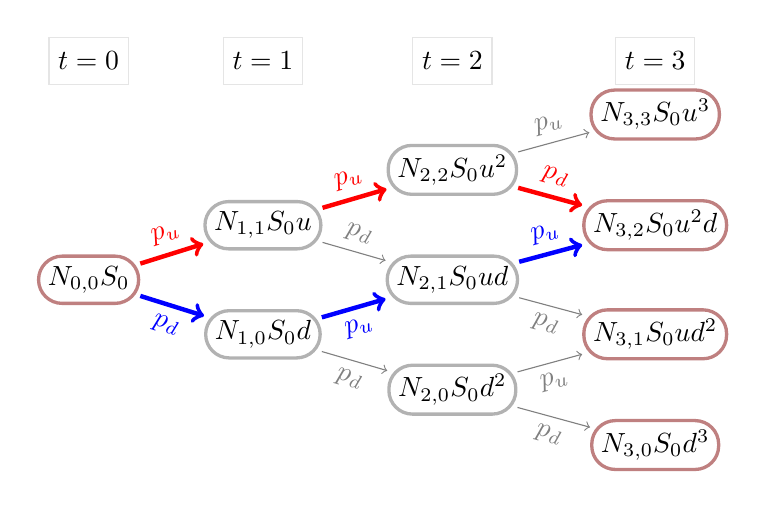
\begin{tikzpicture}
			\matrix[column sep=8mm,row sep=0.4mm,ampersand replacement=\&] (tree){
				\node[header] (t0) {$ t = 0 $};  \&  \node[header] (t1) {$ t = 1 $};  \&  \node[header] (t2) {$ t = 2 $};  \&  \node[header] (t3) {$ t = 3 $};  \\
				\&  \&  \& \node[term] (u3) {$ N_{3,3} \blacktriangleright S_0 u^3 $};  \\
				\&  \&  \node[nterm] (u2) {$ N_{2,2} \blacktriangleright S_0 u^2 $};  \&  \\
				\&  \node[nterm] (u) {$ N_{1,1} \blacktriangleright S_0 u $};  \&  \&  \node[term] (u2d) {$ N_{3,2} \blacktriangleright S_0 u^2 d $};  \\
				\node[term] (s) {$ N_{0,0} \blacktriangleright S_0 $};  \&  \&  \node[nterm] (ud) {$ N_{2,1} \blacktriangleright S_0 u d $};  \&  \\
				\&  \node[nterm] (d) {$ N_{1,0} \blacktriangleright S_0 d $};  \&  \&	\node[term] (ud2) {$ N_{3,1} \blacktriangleright S_0 u d^2 $};  \\
				\&  \&  \node[nterm] (d2) {$ N_{2,0} \blacktriangleright S_0 d^2 $};  \&  \\
				\&  \&  \& \node[term] (d3) {$ N_{3,0} \blacktriangleright S_0 d^3 $};  \\
			};
			
			% Lines out of s
			\draw[->,red,ultra thick] (s) -- (u) node[midway,above,sloped] {$p_u$};
			\draw[->,blue,ultra thick] (s) -- (d) node[midway,below,sloped] {$p_d$};
			% Lines out of u
			\draw[->,red,ultra thick] (u) -- (u2) node[midway,above,sloped] {$p_u$};
			\draw[->,gray] (u) -- (ud) node[midway,above,sloped] {$p_d$};
			% Lines out of d
			\draw[->,blue,ultra thick] (d) -- (ud) node[midway,below,sloped] {$p_u$};
			\draw[->,gray] (d) -- (d2) node[midway,below,sloped] {$p_d$};
			% Lines out of u2
			\draw[->,gray] (u2) -- (u3) node[midway,above,sloped] {$p_u$};
			\draw[->,red,ultra thick] (u2) -- (u2d) node[midway,above,sloped] {$p_d$};
			% Lines out of ud
			\draw[->,blue,ultra thick] (ud) -- (u2d) node[midway,above,sloped] {$p_u$};
			\draw[->,gray] (ud) -- (ud2) node[midway,below,sloped] {$p_d$};
			% Lines out of d2
			\draw[->,gray] (d2) -- (ud2) node[midway,below,sloped] {$p_u$};
			\draw[->,gray] (d2) -- (d3) node[midway,below,sloped] {$p_d$};
			\end{tikzpicture}
			
			%		\caption{A 3-step recombinant tree}
			%		\label{fig:paths}
		\end{figure}
	\end{frame}
	
	
	\begin{frame}{\cite{Black1973} model (continuous)}
		\begin{description}
			\item[riskless] $ S_t^0 = e^{rt} $
			\item[risky] $ S_t  =  s_0 e^{ ( r - \frac{\sigma^2}{2} ) t + \sigma W_t } $
		\end{description}
		
		\begin{theorem}[Convergence of prices from CRR to BS]
			Prices of basic assets under CRR $ \xrightarrow{d} $ prices of basic assets under BS.
		\end{theorem}
		
		\begin{corollary}[Convergence of evaluation formulae]
			The previous theorem implies that evaluation formulae under CRR converge in distribution to evaluation formulae for BS.
		\end{corollary}
		
		\bigskip
		
		Approximate BS price by using CRR model.
		
		\bigskip
		
		\alert{Quest}: Find algorithms with reduced computational complexity.
		
	\end{frame}
	
	
	\begin{frame}{Market models: discrete vs. continuous}
		\begin{tabular}{lll}
			\toprule
			Parameter  &  Discrete  &  Continuous  \\
			\midrule
			Example  &  \cite{Cox1979}  &  \cite{Black1973}  \\
			Theoretical complexity  &  Easy  &  Hard  \\
			Ease of implementation  &  Hard  &  Easy  \\
			Closed-form formula  &  No\footnotemark  &  Yes  \\
			Computational complexity  &  Hard: $ O(2^n) $\footnotemark[1]  &  Easy: $ O(1) $  \\
			Versatile  &  Yes  &  No  \\
			\bottomrule
		\end{tabular}
		\footnotetext{CRR: backward recursive}
	\end{frame}
	
	
	
	\section{Asian options}
	
	\begin{frame}{Asian options: introduction}
		Payoff: function of some form of average price.
		
		\bigskip
		
		\begin{tabular}{lll}
			\toprule
			Average  &  Discrete  &  Continuous  \\
			\midrule
			AM  &  $ A_n = \frac{1}{n+1} \sum_{i=0}^{n} S_n $  &  $ A_T = \frac{1}{T} \int_{0}^{T} S_t \dif t $  \\
			GM  &  $ G_n = \left( \prod_{i=0}^{n} S_n \right)^{\frac{1}{n+1}} $  &  $  
			G_T = \exp \left(  \frac{1}{T} \int_{0}^{T} \log(S_t) \dif t  \right) $  \\
			\bottomrule
		\end{tabular}
		
		\bigskip
		
		\begin{example}[fixed-strike Asian call of European type]
			Given strike-price $ K $, payoff $ = (A_T - K)_+ $, exercised only at maturity.
		\end{example}	
	\end{frame}
	
	
	\begin{frame}{Asian option: pre-existing methods}
		\begin{block}{Arithmetic mean}
			\begin{tabular}{cccl}
				\toprule
				Method  &  Type  &  Complex  &  Remarks  \\
				\midrule
				\cite{Cox1979}  &  Tree  &  \alert{$ O(2^n) $}  &  simple, accurate, convergence  \\
				\cite{Hull1993}  &  Tree  &  $ O(n^3) $  &  accuracy \& convergence problems  \\
				\cite{Barraquand1996}  &  Tree  &  $ O(n^3) $  &  accuracy \& convergence problems  \\
				\cite{Chalasani1999}  &  Tree  &  $ O(n^4) $  &  thin bounds, very large memory  \\
				\cite{Vecer2001}  &  PDE  &  $ O(n^2) $  &  not universally applicable  \\
				\cite{dHalluin2005}  &  PDE  &    &  more general than \cite{Vecer2001} \\
				\bottomrule
			\end{tabular}
		\end{block}
		
		\bigskip
		
		\begin{block}{Geometric mean}
			Closed-form formula exist under BS.
		\end{block}
	\end{frame}
	
	
	\begin{frame}{SPM for Asian options: idea}
		\begin{description}
			\item[$ N_{i,j} $] Node of the binomial tree
			\item[$ A_{i,j}^l $] Average upto $ N_{i,j} $, $ l \in \binom{i}{j} $
			\item[$ P_{i,j}^l $] Corresponding option price
			\item[$ \left\lbrace \left( A_{i,j}^l, P_{i,j}^l \right) \right\rbrace_l $] \alert{singular points} (SPs) -- \alert{completely characterise price}
			\item[price function] continuous, convex, piecewise-linear; found by joining SPs.
		\end{description}
	\end{frame}
	
	
	\begin{frame}{SPM for Asian options: start at maturity ($ i = n $)}
		\begin{minipage}[t]{0.55\linewidth}
			For $ N_{n,j} $: calculate $ A_{i,j}^{\min} $ and $ A_{i,j}^{\max} $.
			
			\bigskip
			
			Singular points:
			\begin{enumerate}
				\item $ j \in \{ 0, n \} $: $ (A, (A-K)_+) $
				\item $ j \notin \{ 0, n \} $ and $ K \in \left( A_{n,j}^{\min}, A_{n,j}^{\max} \right) $: \begin{enumerate}
					\item $ ( A_{n,j}^{\min} , 0 ) $
					\item $ ( K , 0 ) $
					\item $ ( A_{n,j}^{\max} , A_{n,j}^{\max} - K ) $
				\end{enumerate}
				\item $ j \notin \{ 0, n \} $ and $ K \notin \left( A_{n,j}^{\min}, A_{n,j}^{\max} \right) $:
				\begin{enumerate}
					\item $ \left( A_{n,j}^{\min} , ( A_{n,j}^{\min} - K )_+ \right) $
					\item $ \left( A_{n,j}^{\max} , ( A_{n,j}^{\max} - K )_+ \right) $
				\end{enumerate}
			\end{enumerate}
		\end{minipage}
		\begin{minipage}[t]{0.40\linewidth}
			\begin{figure}
				\definecolor{qqwwtt}{rgb}{0.,0.4,0.2}
				\definecolor{ffqqqq}{rgb}{1.,0.,0.}
				\definecolor{zzttqq}{rgb}{0.6,0.2,0.}
				\begin{tikzpicture}[line cap=round,line join=round,>=triangle 45,x=1.0cm,y=1.0cm]
				\draw[->,color=black] (-0.5,0.) -- (3.5,0.);
				\foreach \x in {,1.,2.,3.}
				\draw[shift={(\x,0)},color=black] (0pt,2pt) -- (0pt,-2pt);
				\draw[color=black] (3.263006775519728,0.05820970293171456) node [anchor=south west] { A};
				\draw[->,color=black] (0.,-0.5) -- (0.,2.);
				\foreach \y in {,1.}
				\draw[shift={(0,\y)},color=black] (2pt,0pt) -- (-2pt,0pt);
				\draw[color=black] (0.0727621286646436,1.673064914416971) node [anchor=west] { P};
				\clip(-0.5,-0.5) rectangle (3.5,2.);
				\draw [line width=2.pt,color=ffqqqq] (1.5167156875682812,0.)-- (3.,1.5);
				\draw [line width=0.4pt,dash pattern=on 1pt off 1pt,color=qqwwtt] (3.,1.5)-- (3.,0.);
				\draw [line width=2.pt,color=ffqqqq] (0.49804588626327045,0.)-- (1.5167156875682812,0.);
				\draw [line width=0.4pt,dash pattern=on 1pt off 1pt,color=qqwwtt] (3.,1.5)-- (0.,1.4984358056218274);
				\begin{scriptsize}
				\draw [fill=zzttqq] (1.5167156875682812,0.) circle (2.5pt);
				\draw[color=zzttqq] (1.5167156875682817,-0.3642746881930386) node {$K$};
				\draw [fill=zzttqq] (3.,1.5) circle (2.5pt);
				\draw [fill=qqwwtt] (3.,0.) circle (2.0pt);
				\draw[color=qqwwtt] (3.0156155380599396,-0.2769601337954668) node {$A_{i,j}^{\max}$};
				\draw [fill=zzttqq] (0.49804588626327045,0.) circle (2.5pt);
				\draw[color=zzttqq] (0.6290177178596299,-0.32061741099425267) node {$A_{i,j}^{\min}$};
				\draw [fill=qqwwtt] (0.,1.4984358056218274) circle (2.0pt);
				\draw[color=qqwwtt] (0.8618565295864893,1.2219397166961832) node {$\left( A_{i,j}^{\max} - K \right)_+$};
				\end{scriptsize}
				\end{tikzpicture}
				
				\caption{Case 2}
			\end{figure}		
		\end{minipage}
	\end{frame}
	
	
	\begin{frame}{SPM for Asian options: exact price}
		\begin{minipage}[t]{0.6\linewidth}
			\begin{itemize}
				\item Up movement (for $ N_{i,j} $):
				\begin{enumerate}
					\item $ \forall A_{i+1,j}^l: B^l = \frac{ ( i+2) A_{i+1,j}^l - S_{i+1,j} }{ i+1 } $.
					\item If $ B^l \in \left[ A_{i,j}^{\min}, A_{i,j}^{\max} \right]  \implies B^l $ is SA.
					\item For each SA, $ B^l_u = \frac{(i+1) B^l + S_{i+1,j+1}}{i+2} $.
					\item $ v_{i,j}( B^l ) = \frac{1}{R} \left[ p_u v_{i+1,j+1} \left( B^l_u \right) + p_d v_{i+1,j} \left( A_{i+1,j}^l \right) \right] $.
					\item $ \left( B^l, v_{i,j}( B^l ) \right) $ is a SP.
				\end{enumerate}
				\item Down movement (for $ N_{i,j} $).
				\item Aggregate and sort by SAs.
				\item Repeat for all $ j $.
				\item Iterate backward till $ i = 0 $. $ P_{0,0}^1 $ is the exact binomial price.
			\end{itemize}
			
		\end{minipage}
		\begin{minipage}[t]{0.3\linewidth}
			\begin{figure}
				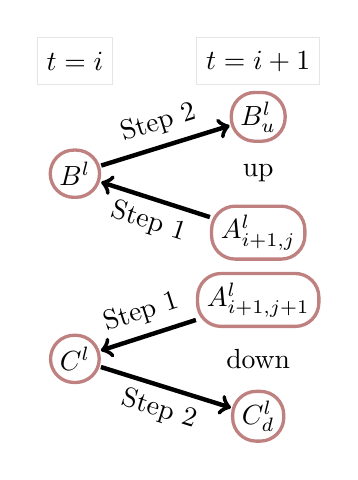
\begin{tikzpicture}
				\matrix (tree) [column sep=3em,row sep=0.2em,ampersand replacement=\&]{
					\node[header] (t0) {$ t = i $};  \&  \node[header] (t1) {$ t = i+1 $};  \\
					\&  \node[term] (u-u) {$ B^l_u $};  \\
					\node[term] (u-s) {$ B^l $};  \&  \node {up};  \\
					\&  \node[term] (u-d) {$ A_{i+1,j}^l $};  \\
					\\
					\&  \node[term] (d-u) {$ A_{i+1,j+1}^l $};  \\
					\node[term] (d-s) {$ C^l $};  \&  \node {down};  \\
					\&  \node[term] (d-d) {$ C^l_d $}; \\
				};
				\draw[->,ultra thick] (u-s) -- (u-u) node[midway,above,sloped] {Step 2};
				\draw[->,ultra thick] (u-d) -- (u-s) node[midway,below,sloped] {Step 1};
				\draw[->,ultra thick] (d-u) -- (d-s) node[midway,above,sloped] {Step 1};
				\draw[->,ultra thick] (d-s) -- (d-d) node[midway,below,sloped] {Step 2};
				\end{tikzpicture}
			\end{figure}
		\end{minipage}
	\end{frame}
	
	
	\begin{frame}{SPM for Asian options: approximation}{Upper estimates}
		\definecolor{qqqqff}{rgb}{0.,0.,1.}
		\definecolor{wqwqwq}{rgb}{0.3764705882352941,0.3764705882352941,0.3764705882352941}
		\definecolor{qqwwtt}{rgb}{0.,0.4,0.2}
		\definecolor{ffqqqq}{rgb}{1.,0.,0.}
		\definecolor{zzttqq}{rgb}{0.6,0.2,0.}
		\begin{tikzpicture}[line cap=round,line join=round,>=triangle 45,x=0.5894736842105263cm,y=0.45cm]
		\draw[->,color=black] (0.,0.) -- (18.,0.);
		\foreach \x in {,2.,4.,6.,8.,10.,12.,14.,16.}
		\draw[shift={(\x,0)},color=black] (0pt,2pt) -- (0pt,-2pt);
		\draw[color=black] (17.488266365982355,0.12712930521358398) node [anchor=south west] { A};
		\draw[->,color=black] (0.,0.) -- (0.,13.);
		\foreach \y in {,2.,4.,6.,8.,10.,12.}
		\draw[shift={(0,\y)},color=black] (2pt,0pt) -- (-2pt,0pt);
		\draw[color=black] (0.158911605284918,12.306834374720044) node [anchor=west] { P};
		\clip(-1.,-1.) rectangle (18.,13.);
		\draw [line width=2.pt,color=ffqqqq] (16.,12.)-- (12.05,7.25);
		\draw [line width=2.pt,color=ffqqqq] (8.,4.)-- (4.,2.5);
		\draw [line width=2.pt,color=ffqqqq] (4.,2.5)-- (1.,2.);
		\draw [line width=0.4pt,color=wqwqwq] (12.05,7.25)-- (12.,0.);
		\draw [line width=0.4pt,color=wqwqwq] (8.,4.)-- (8.,0.);
		\draw [line width=0.4pt,color=wqwqwq] (4.,2.5)-- (4.,0.);
		\draw [line width=0.4pt,color=wqwqwq] (1.,2.)-- (1.,0.);
		\draw [line width=2.pt,dash pattern=on 1pt off 1pt on 2pt off 4pt,color=qqqqff] (4.,2.5)-- (12.05,7.25);
		\draw [line width=0.4pt,color=wqwqwq] (16.,12.)-- (16.,0.);
		\draw [line width=1.2pt,dotted,color=qqwwtt] (8.004137964992687,4.862690103567112)-- (8.,4.);
		\draw [line width=2.pt,color=ffqqqq] (8.,4.)-- (12.05,7.25);
		\draw (2.487010827086094,9.891377575661947) node[anchor=north west] {$f_u(A) \ge f(A) \quad \forall A$};
		\draw (2.518793148143078,8.397608239402336) node[anchor=north west] {$(f_u - f)(A) \le \varepsilon \quad \forall A$};
		\begin{scriptsize}
		\draw [fill=zzttqq] (16.,12.) circle (2.0pt);
		\draw[color=zzttqq] (16.40766745004491,11.512276217135144) node {$S_5$};
		\draw [fill=zzttqq] (12.05,7.25) circle (2.0pt);
		\draw[color=zzttqq] (12.434877317921963,6.840274250535932) node {$S_4$};
		\draw [fill=zzttqq] (8.,4.) circle (2.0pt);
		\draw[color=zzttqq] (8.36674022262806,3.5349123149827486) node {$S_3$};
		\draw [fill=zzttqq] (4.,2.5) circle (2.0pt);
		\draw[color=zzttqq] (4.362167769448127,2.041142978723137) node {$S_2$};
		\draw[color=ffqqqq] (6.300889353924126,2.9946127678250165) node {f};
		\draw [fill=zzttqq] (1.,2.) circle (2.0pt);
		\draw[color=zzttqq] (1.4064119111486517,1.6915373893857808) node {$S_1$};
		\draw [fill=qqwwtt] (16.,0.) circle (2.0pt);
		\draw[color=qqwwtt] (16.185191202646024,-0.43787847294175086) node {$A_5$};
		\draw [fill=qqwwtt] (12.,0.) circle (2.0pt);
		\draw[color=qqwwtt] (12.117054107352125,-0.4696607992451468) node {$A_4$};
		\draw [fill=qqwwtt] (8.,0.) circle (2.0pt);
		\draw[color=qqwwtt] (8.080699333115207,-0.5332254518519388) node {$A_3$};
		\draw [fill=qqwwtt] (4.,0.) circle (2.0pt);
		\draw[color=qqwwtt] (4.04434455887829,-0.5650077781553349) node {$A_2$};
		\draw [fill=qqwwtt] (1.,0.) circle (2.0pt);
		\draw[color=qqwwtt] (1.056806379521832,-0.5332254518519388) node {$A_1$};
		\draw[color=qqqqff] (9.002386643767732,6.109280745557824) node {$f_u$};
		\draw [fill=qqqqff] (8.004137964992687,4.862690103567112) circle (2.0pt);
		\draw[color=qqqqff] (7.508617554089503,5.092246303849152) node {$R_3$};
		\draw[color=qqwwtt] (8.36674022262806,4.488382104084628) node {$\varepsilon$};
		\draw[color=ffqqqq] (10.432591091331993,5.5054165457933) node {f};
		\end{scriptsize}
		\end{tikzpicture}
	\end{frame}
	
	
	\begin{frame}{SPM for Asian options: approximation}{Lower estimates}
		\definecolor{wqwqwq}{rgb}{0.3764705882352941,0.3764705882352941,0.3764705882352941}
		\definecolor{qqwwtt}{rgb}{0.,0.4,0.2}
		\definecolor{ffqqqq}{rgb}{1.,0.,0.}
		\definecolor{qqqqff}{rgb}{0.,0.,1.}
		\definecolor{zzttqq}{rgb}{0.6,0.2,0.}
		\begin{tikzpicture}[line cap=round,line join=round,>=triangle 45,x=0.59cm,y=0.45cm]
		\draw[->,color=black] (0.,0.) -- (17.,0.);
		\foreach \x in {,2.,4.,6.,8.,10.,12.,14.,16.}
		\draw[shift={(\x,0)},color=black] (0pt,2pt) -- (0pt,-2pt);
		\draw[color=black] (16.35554728730377,0.15704689406799202) node [anchor=south west] { A};
		\draw[->,color=black] (0.,0.) -- (0.,13.);
		\foreach \y in {,2.,4.,6.,8.,10.,12.}
		\draw[shift={(0,\y)},color=black] (2pt,0pt) -- (-2pt,0pt);
		\draw[color=black] (0.19630858508193877,12.12903270711778) node [anchor=west] { P};
		\clip(-1.,-1.) rectangle (17.,13.);
		\draw [line width=2.pt,color=qqqqff] (4.,2.5)-- (12.,8.);
		\draw [line width=2.pt,color=ffqqqq] (16.,12.)-- (12.,8.);
		\draw [line width=0.4pt,color=wqwqwq] (12.,8.)-- (12.,0.);
		\draw [line width=0.4pt,color=wqwqwq] (4.,2.5)-- (4.,0.);
		\draw [line width=0.4pt,color=wqwqwq] (1.,2.)-- (1.,0.);
		\draw [line width=2.pt,dash pattern=on 4pt off 4pt,color=ffqqqq] (4.,2.5)-- (7.,3.);
		\draw [line width=2.pt,dash pattern=on 4pt off 4pt,color=ffqqqq] (12.,8.)-- (7.,3.);
		\draw [line width=0.4pt,color=wqwqwq] (7.,3.)-- (6.998942733420039,0.);
		\draw [line width=0.4pt,color=wqwqwq] (16.,12.)-- (16.,0.);
		\draw [line width=1.2pt,dash pattern=on 2pt off 2pt,color=qqwwtt] (7.000519372007349,4.562857068255052)-- (7.,3.);
		\draw (1.9857588593058553,11.54010685436281) node[anchor=north west] {$f_d(A) \le f(A) \quad \forall A$};
		\draw (1.9857588593058553,10.480040319403864) node[anchor=north west] {$(f - f_d) (A) \le \varepsilon  \quad  \forall A$};
		\draw [line width=2.pt,color=ffqqqq] (1.,2.)-- (4.,2.5);
		\begin{scriptsize}
		\draw [fill=zzttqq] (16.,12.) circle (2.0pt);
		\draw[color=zzttqq] (16.355547287303775,11.50084513084581) node {$S_4$};
		\draw [fill=zzttqq] (12.,8.) circle (2.0pt);
		\draw[color=zzttqq] (12.429375585664998,7.260578991010027) node {$S_3$};
		\draw [fill=zzttqq] (4.,2.5) circle (2.0pt);
		\draw[color=zzttqq] (4.4592470313382835,2.038769763249292) node {$S_2$};
		\draw [fill=zzttqq] (1.,2.) circle (2.0pt);
		\draw[color=zzttqq] (1.2790479530108758,1.528367357528318) node {$S_1$};
		\draw [fill=qqwwtt] (16.,0.) circle (2.0pt);
		\draw[color=qqwwtt] (16.041453551172673,-0.7095508829405683) node {$A_4$};
		\draw [fill=qqwwtt] (12.,0.) circle (2.0pt);
		\draw[color=qqwwtt] (12.076020132517508,-0.6702891594235703) node {$A_3$};
		\draw [fill=qqwwtt] (4.,0.) circle (2.0pt);
		\draw[color=qqwwtt] (4.105891578190794,-0.6702891594235703) node {$A_2$};
		\draw [fill=qqwwtt] (1.,0.) circle (2.0pt);
		\draw[color=qqwwtt] (1.0042159338961614,-0.7488126064575662) node {$A_1$};
		\draw [fill=qqwwtt] (6.998942733420039,0.) circle (2.0pt);
		\draw[color=qqwwtt] (7.011258637403488,-0.7095508829405683) node {$A_{23}$};
		\draw [fill=ffqqqq] (7.,3.) circle (2.0pt);
		\draw[color=ffqqqq] (7.482399241600141,2.1565549338002863) node {$R_{23}$};
		\draw[color=ffqqqq] (5.833407126911855,2.1565549338002863) node {$f_d$};
		\draw[color=ffqqqq] (9.798840545567018,4.944137303507144) node {$f_d$};
		\draw [fill=qqqqff] (7.000519372007349,4.562857068255052) circle (2.0pt);
		\draw[color=qqqqff] (6.5793797502232225,5.925680391432095) node {$S_{23}$};
		\draw[color=qqwwtt] (7.875016411764018,3.7270238744802064) node {$\varepsilon_4$};
		\end{scriptsize}
		\end{tikzpicture}
	\end{frame}
	
	
	\begin{frame}{SPM for Asian options: numerical results}
		Data: $ s_0 = 100, T = 1, r = 0.1, q = 0.03 $.
		\begin{tabular}{crcccc}
			\toprule
			&         &  \multicolumn{2}{c}{$ K = 90 $}  &  \multicolumn{2}{c}{$ K = 110 $}  \\
			\cmidrule(lr){3-4}\cmidrule(lr){5-6}
			&  $ n $  &  $ \sigma = 0.2 $  &  $ \sigma = 0.4 $  &  $ \sigma = 0.2 $  &  $ \sigma = 0.4 $  \\
			\midrule
			\multirow{2}{2em}{Bin}
			&   10  &  14.5912  &  17.8033  &  2.5100  &  6.6523  \\
			&   25  &  15.1535  &  18.6786  &  2.6270  &  7.3451  \\
			\midrule
			\multirow{6}{2em}{SP}
			&   10  &  14.5925  &  17.8068  &  2.5090  &  6.6511  \\
			&   25  &  15.1535  &  18.6785  &  2.6270  &  7.3449  \\
			&   50  &  15.3524  &  19.0420  &  2.6673  &  7.4563  \\
			&  100  &  15.4732  &  19.2696  &  2.6886  &  7.5174  \\
			&  200  &  15.5453  &  19.4065  &  2.6996  &  7.5502  \\
			&  400  &  15.5861  &  19.4845  &  2.7053  &  7.5674  \\
			\bottomrule
		\end{tabular}
	\end{frame}
	
	
	\begin{frame}{SPM for Asian options: summary}
		\begin{itemize}
			\neu Introduced by Gaudenzi \emph{et al} \cite{Gaudenzi2010} in 2010.
			\pro Convergent to exact CRR and thus BS.
			\pro Easily generalised to American case and lookback options.
			\pro Approx: unnecessary points $ \implies $ selective removal.
			\pro Approx: \emph{A priori} error bounds.
			\pro Approx $ \implies $ fast: reduction of complexity from exponential time to polynomial time (experimental) of $ O(n^3) $.
			\con Difficult to compute theoretical complexity.
			\con Depends on the recombinant nature of the underlying's tree.
			\con<alert@1-> Not extensible to GM, since the price function is non-linear. $ G_u = \left( G^{i+1} S_{i+1,j} \right)^{\frac{1}{i+2}} \propto G^{\frac{i+1}{i+2}} $
			\con<alert@1-> Constant volatility assumption $ \implies $ local volatility models fail.
		\end{itemize}
	\end{frame}
	
	
	
	\section{Cliquet options}
	
	\begin{frame}{Cliquet options: introduction}
		\begin{block}{Definitions}
			\begin{description}
				\item[forward start option] price option today with payoff $ = (S_T - S_u)_+ $, $ 0 \le u < T $.
				\item[cliquet option] a series of consecutive at-the-money forward start options, with bounded returns.
			\end{description}
		\end{block}
		\begin{block}{Pre-existing methods for pricing}
			\begin{itemize}
				\item No prominent tree-based method.
				\item \cite{Wilmott2002}: PDE based, FD approach.
				\item \cite{Windcliff2006}: PDE based, FD approach; generalisations.
			\end{itemize}
		\end{block}
	\end{frame}
	
	
	\begin{frame}{Cliquet options: terminology}
		\begin{itemize}
			\item $ N $: observation times (equidistant).
			\item Return: $ R_i = \frac{S_i - S_{i-1}}{S_{i-1}} = \frac{S_i}{S_{i-1}} - 1 $.
			\item Running sum: $ Z_i = \sum_{k = 1}^{i} \max \{ F_{loc}, \min \{ C_{loc}, R_k \} \} $.
			\item Payoff = $ \max \{ F_{glob}, \min \{ C_{glob}, Z_{N} \} \} $.
		\end{itemize}
		
		\begin{minipage}{0.55\textwidth}
			\begin{itemize}
				\item $ m $: computational time steps.
				\item $ 2^m $ possible paths; $ \sim \text{Bin}(p) $.
				\item $ Z $ depends on paths, probs.
				\item $ (Z, P) \implies $ SP ($ P $ is price).
				\item<alert@1-> Price function at maturity.
				\item Proceed as in the Asian case.
				\item Iterate backwards. $ P_0^1 $ is the exact binomial price.
			\end{itemize}
		\end{minipage}
		\begin{minipage}{0.4\textwidth}
			\definecolor{wqwqwq}{rgb}{0.3764705882352941,0.3764705882352941,0.3764705882352941}
			\definecolor{qqwwtt}{rgb}{0.,0.4,0.2}
			\definecolor{ffqqqq}{rgb}{1.,0.,0.}
			\definecolor{zzttqq}{rgb}{0.6,0.2,0.}
			\begin{tikzpicture}[line cap=round,line join=round,>=triangle 45,x=0.8cm,y=0.8cm]
			\draw[->,color=black] (0.,0.) -- (5.5,0.);
			\foreach \x in {,1.,2.,3.,4.,5.}
			\draw[shift={(\x,0)},color=black] (0pt,2pt) -- (0pt,-2pt);
			\draw[color=black] (5.2791785799460476,0.054247335995569544) node [anchor=south west] { Z};
			\draw[->,color=black] (0.,0.) -- (0.,3.5);
			\foreach \y in {,1.,2.,3.}
			\draw[shift={(0,\y)},color=black] (2pt,0pt) -- (-2pt,0pt);
			\draw[color=black] (0.06780919373316127,3.2068898782737656) node [anchor=west] { P};
			\clip(-0.5,-1.) rectangle (5.5,3.5);
			\draw [line width=2.pt,color=ffqqqq] (1.,1.)-- (2.,1.);
			\draw [line width=2.pt,color=ffqqqq] (2.,1.)-- (4.,3.);
			\draw [line width=2.pt,color=ffqqqq] (4.,3.)-- (5.,3.);
			\draw [line width=0.4pt,color=wqwqwq] (1.,1.)-- (1.,0.);
			\draw [line width=0.4pt,color=wqwqwq] (2.,1.)-- (2.,0.);
			\draw [line width=0.4pt,color=wqwqwq] (4.,3.)-- (4.,0.);
			\draw [line width=0.4pt,color=wqwqwq] (5.,3.)-- (5.,0.);
			\draw [line width=0.4pt,color=wqwqwq] (1.,1.)-- (0.,1.);
			\draw [line width=0.4pt,color=wqwqwq] (4.,3.)-- (0.,3.);
			\begin{scriptsize}
			\draw [fill=zzttqq] (1.,1.) circle (2.5pt);
			\draw[color=zzttqq] (0.9258283422770939,1.4438514584177555) node {$S_1$};
			\draw [fill=zzttqq] (2.,1.) circle (2.5pt);
			\draw[color=zzttqq] (1.7666623445682936,1.4438514584177555) node {$S_2$};
			\draw [fill=zzttqq] (4.,3.) circle (2.5pt);
			\draw[color=zzttqq] (4.2077933189621,2.6237310163213934) node {$S_3$};
			\draw [fill=zzttqq] (5.,3.) circle (2.5pt);
			\draw[color=zzttqq] (5.170683869972989,2.6644165183180704) node {$S_4$};
			\draw [fill=qqwwtt] (1.,0.) circle (1.5pt);
			\draw[color=qqwwtt] (0.8580191485439326,-0.3191869614382546) node {$F_{loc} N_{obs}$};
			\draw [fill=qqwwtt] (2.,0.) circle (1.5pt);
			\draw[color=qqwwtt] (2.065022796994203,-0.3191869614382546) node {$F_{glob}$};
			\draw [fill=qqwwtt] (4.,0.) circle (1.5pt);
			\draw[color=qqwwtt] (3.963680221522719,-0.3191869614382546) node {$C_{glob}$};
			\draw [fill=qqwwtt] (5.,0.) circle (1.5pt);
			\draw[color=qqwwtt] (5.035065482506667,-0.3191869614382546) node {$C_{loc} N_{obs}$};
			\draw [fill=qqwwtt] (0.,1.) circle (1.5pt);
			\draw[color=qqwwtt] (-0.17268059620011877,0.8742544304642753) node {$F_{glob}$};
			\draw [fill=qqwwtt] (0.,3.) circle (1.5pt);
			\draw[color=qqwwtt] (-0.22692795118664777,2.908529530298133) node {$C_{glob}$};
			\end{scriptsize}
			\end{tikzpicture}
		\end{minipage}
		
	\end{frame}
	
	
	\begin{frame}{SPM for cliquet options: approximation}
		\definecolor{ffffqq}{rgb}{1.,1.,0.}
		\definecolor{dqfqcq}{rgb}{0.8156862745098039,0.9411764705882353,0.7529411764705882}
		\definecolor{wqwqwq}{rgb}{0.3764705882352941,0.3764705882352941,0.3764705882352941}
		\definecolor{afeeee}{rgb}{0.6862745098039216,0.9333333333333333,0.9333333333333333}
		\definecolor{ffffff}{rgb}{1.,1.,1.}
		\begin{tikzpicture}[line cap=round,line join=round,>=triangle 45,x=0.59cm,y=0.45cm]
		\draw[->,color=ffffff] (0.,0.) -- (17.,0.);
		\foreach \x in {,2.,4.,6.,8.,10.,12.,14.,16.}
		\draw[shift={(\x,0)},color=ffffff] (0pt,2pt) -- (0pt,-2pt);
		\draw[color=ffffff] (17.71074261338124,0.12712930521358398) node [anchor=south west] { A};
		\draw[->,color=ffffff] (0.,0.) -- (0.,13.);
		\foreach \y in {,2.,4.,6.,8.,10.,12.}
		\draw[shift={(0,\y)},color=ffffff] (2pt,0pt) -- (-2pt,0pt);
		\draw[color=ffffff] (0.158911605284918,12.052575764292875) node [anchor=west] { P};
		\clip(-1.,-1.) rectangle (17.,13.);
		\draw [line width=2.pt,color=afeeee] (16.,12.)-- (12.05,7.25);
		\draw [line width=2.pt,color=afeeee] (8.,3.75)-- (4.,2.5);
		\draw [line width=2.pt,color=afeeee] (4.,2.5)-- (1.,2.);
		\draw [line width=0.4pt,color=wqwqwq] (12.05,7.25)-- (12.,0.);
		\draw [line width=0.4pt,color=wqwqwq] (8.,3.75)-- (8.,0.);
		\draw [line width=0.4pt,color=wqwqwq] (4.,2.5)-- (4.,0.);
		\draw [line width=0.4pt,color=wqwqwq] (1.,2.)-- (1.,0.);
		\draw [line width=2.pt,dash pattern=on 1pt off 1pt on 2pt off 4pt,color=dqfqcq] (4.,2.5)-- (12.05,7.25);
		\draw [line width=0.4pt,color=wqwqwq] (16.,12.)-- (16.,0.);
		\draw [line width=1.2pt,dotted,color=ffffqq] (8.025,4.875)-- (8.,3.75);
		\draw [line width=2.pt,color=afeeee] (8.,3.75)-- (12.05,7.25);
		\draw [color=dqfqcq](2.487010827086094,9.891377575661947) node[anchor=north west] {$f_u(A) \ge f(A) \quad \forall A$};
		\draw [color=ffffqq](2.518793148143078,8.397608239402336) node[anchor=north west] {$(f_u - f)(A) \le \varepsilon \quad \forall A$};
		\begin{scriptsize}
		\draw [fill=afeeee] (16.,12.) circle (2.0pt);
		\draw[color=afeeee] (16.40766745004491,11.512276217135144) node {$S_5$};
		\draw [fill=afeeee] (12.05,7.25) circle (2.0pt);
		\draw[color=afeeee] (12.434877317921963,6.840274250535932) node {$S_4$};
		\draw [fill=afeeee] (8.,3.75) circle (2.0pt);
		\draw[color=afeeee] (8.36674022262806,3.280653704555581) node {$S_3$};
		\draw [fill=afeeee] (4.,2.5) circle (2.0pt);
		\draw[color=afeeee] (4.362167769448127,2.041142978723137) node {$S_2$};
		\draw[color=afeeee] (6.3326716749811105,2.8674834626114327) node {f};
		\draw [fill=afeeee] (1.,2.) circle (2.0pt);
		\draw[color=afeeee] (1.4064119111486517,1.6915373893857808) node {$S_1$};
		\draw [fill=afeeee] (16.,0.) circle (2.0pt);
		\draw[color=afeeee] (16.185191202646024,-0.43787847294175086) node {$A_5$};
		\draw [fill=afeeee] (12.,0.) circle (2.0pt);
		\draw[color=afeeee] (12.117054107352125,-0.4696607992451468) node {$A_4$};
		\draw [fill=afeeee] (8.,0.) circle (2.0pt);
		\draw[color=afeeee] (8.080699333115207,-0.5332254518519388) node {$A_3$};
		\draw [fill=afeeee] (4.,0.) circle (2.0pt);
		\draw[color=afeeee] (4.04434455887829,-0.5650077781553349) node {$A_2$};
		\draw [fill=afeeee] (1.,0.) circle (2.0pt);
		\draw[color=afeeee] (1.056806379521832,-0.5332254518519388) node {$A_1$};
		\draw[color=dqfqcq] (9.002386643767732,6.109280745557824) node {$f_u$};
		\draw [fill=dqfqcq] (8.025,4.875) circle (2.0pt);
		\draw[color=dqfqcq] (7.508617554089503,5.092246303849152) node {$R_3$};
		\draw[color=ffffqq] (8.36674022262806,4.361252798871044) node {$\varepsilon$};
		\draw[color=afeeee] (10.432591091331993,5.3782872405797155) node {f};
		\end{scriptsize}
		\end{tikzpicture}
	\end{frame}
	
	
	\begin{frame}{SPM for cliquet options: numerical results}
		\begin{block}{Data}
			\begin{itemize}
				\item $ F_{loc} = 0, C_{loc} = 0.08, F_{glob} = 0.16, C_{glob} = \infty $
				\item $ T = 5, N = 5, r = 0.03 $
			\end{itemize}
		\end{block}
		
		\begin{tabular}{rrcccc}
			\toprule\multirow{2}{1em}{$ \sigma $}  &  \multirow{2}{1em}{$ m $}
			&  \multicolumn{2}{c}{Price}  &  \multicolumn{2}{c}{Time (s)}\footnote{$ \infty $ means time taken is more than an hour.}  \\
			\cmidrule(lr){3-4}\cmidrule(lr){5-6}
			&&  Bin  &  SP  &  Bin  &  SP  \\
			\midrule
			\multirow{3}{1em}{$ 0.2 $}
			&   200  &  0.173716366  &  0.173716366  &  0.0165  &  0.00828  \\
			&   500  &  0.173922597  &  0.173922671  &  0.0875  &  0.0437  \\
			&  1000  &  0.174051949  &  0.174051983  &  2.38  &  0.183  \\
			\midrule
			\multirow{3}{1em}{$ 0.02 $}
			&   200  &  0.150465004  &  0.150466828  &  600  &  6.09  \\
			&   500  &  0.150508871  &  0.150510526  &  $ \infty $  &  24.2  \\
			&  1000  &  0.150522368  &  0.150524027  &  $ \infty $  &  55  \\
			\bottomrule
		\end{tabular}	
	\end{frame}
	
	
	\begin{frame}{SPM for cliquet options: complexity $ O(m^2) $}
		% This plot was generated by plotly
		\begin{figure}
			\centering
			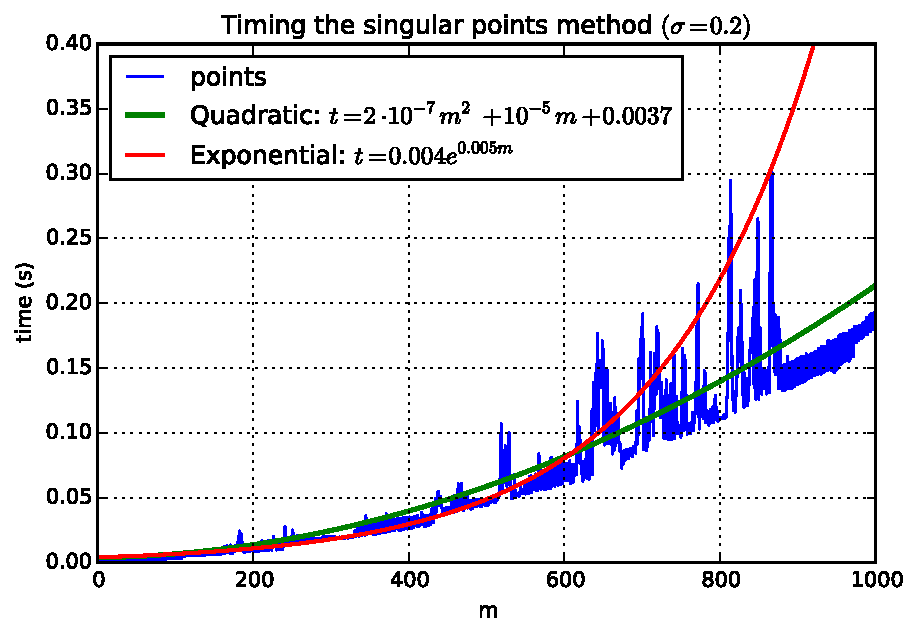
\includegraphics[height=0.75\textheight,width=\textwidth]{../img/timing-cliquet}
		\end{figure}
	\end{frame}
	
	
	\begin{frame}{SPM for cliquet options: summary}
		\begin{itemize}
			\pro Approximation: \emph{A priori} error bounds.
			\con<alert@1-> Approximation: converges to binomial price, no bounds.
			\pro Significant speed improvement in low volatility cases against binomial model.
			\pro<alert@1-> Can be used for local volatility models and varying interest rates in each period.
			\pro<alert@1-> Fast -- experimental order of complexity $ O(m^2) $.
			\con Difficult to compute theoretical complexity.
		\end{itemize}
	\end{frame}
	
	
	\section{Conclusion}
	
	\begin{frame}{Recapitulation}
		\begin{itemize}
			\item Efficient polynomial-time technique.
			\item Theory and flexibility varies with option type.
		\end{itemize}
		
		Further research
		\begin{itemize}
			\item Theoretical complexity: dependence of singular point redundancy on initial data.
			\item Verify cliquet complexity for large $ m $.
			\item Customising the method for other path-dependent options.
		\end{itemize}
	\end{frame}
	
	
	\begin{frame}[plain,c]
		
		\begin{center}
			{\Huge Questions?}
		\end{center}
		
		\vfill
		
		\begin{center}
			{\Huge Thank you!}
		\end{center}
		
	\end{frame}
	
	
	
	\appendix
	
	\begin{frame}<presentation>[allowframebreaks]{Bibliography}
		\printbibliography
	\end{frame}
	
	
\end{document}
